\subsection{Kinds of Models}\label{subsec:KindsofModels}


\begin{frame}{Kinds of Models}    \framesubtitle{Natural and formal languages}


    \AddToShipoutPictureFG*{
        \AtPageUpperLeft{\put(-5,-15){\makebox[\paperwidth][r]{Requirement 1}}}  
        }%


\begin{onlyenv}<1>
    \begin{center}
\begin{figure}
    \centering
    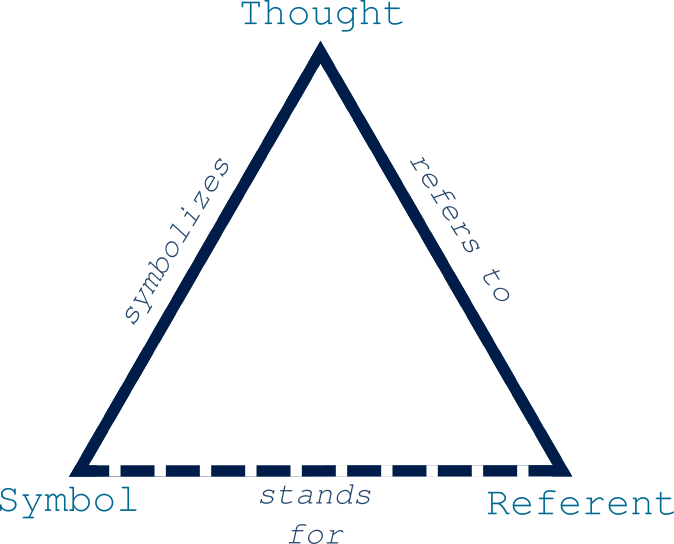
\includegraphics[height =0.5 \textheight, keepaspectratio]{slides/kinds/semantic-triangle/figs/SemanticTriangle.png}
    \caption{Semantic Triangle}
    \label{fig:SemanticTriangle}
\end{figure}
\end{center}
\end{onlyenv}

\begin{onlyenv}<2>
    \begin{center}
\begin{figure}
    \centering
    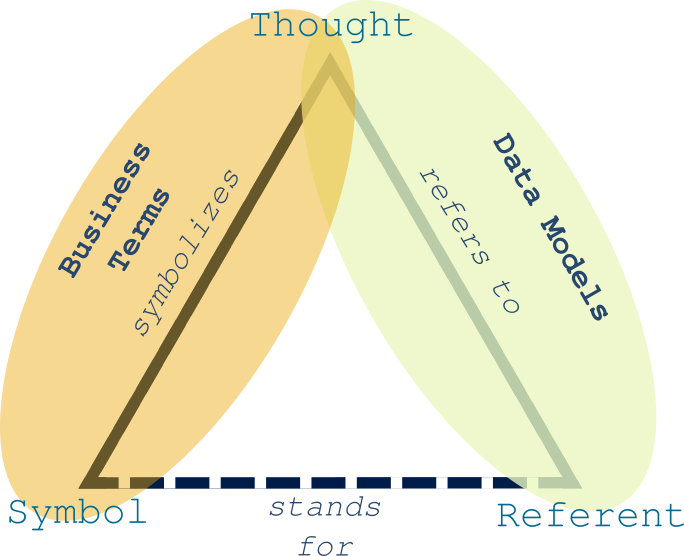
\includegraphics[height =0.5 \textheight, keepaspectratio]{slides/kinds/semantic-triangle/figs/SemanticTriangleModels.png}
    \caption{Semantic Triangle}
    
\end{figure}
\end{center}
\end{onlyenv}
  
\end{frame}